\documentclass[final]{beamer}
\mode<presentation> {
  \usetheme[mat]{HYposter}
}

% Change faculty colours on line 3 by setting \usetheme[<id>]{HYposter}.
% The different faculty ids are:
%  maa: Faculty of Agriculture and Forestry 
%  hum: Faculty of Arts 
%  kay: Faculty of Behavioural Sciences 
%  bio: Faculty of Biological and Environmental Sciences 
%  oik: Faculty of Law 
%  med: Faculty of Medicine 
%  far: Faculty of Pharmacy 
%  mat: Faculty of Science 
%  val: Faculty of Social Sciences 
%  teo: Faculty of Theology 
%  ell: Faculty of Veterinary Medicine 
%  soc: Swedish School of Social Science 
% Without options a black theme without faculty name will be used.

\usepackage[english]{babel}
\usepackage[T1]{fontenc}
\usepackage[utf8]{inputenc}
\usepackage{lmodern}
\usepackage{amsmath,amsthm, amssymb, latexsym}
\usepackage[orientation=portrait,size=a0,scale=1.4,debug]{beamerposter}

% Set up the title and author info
\titlestart{Pretty posters with \LaTeX}
\titleend{using the HYposter style}
\author[Wilkman]{Olli Wilkman}
\institute[University of Helsinki]{}
\date{\today}


\begin{document}
\begin{frame}[t, fragile]
\begin{columns}[T]
	
% First column starts here
\begin{column}{0.32\linewidth}


\begin{block}{\LaTeX~POSTERS MADE EASIER}
The \texttt{HYposter} style enables you to make scientific posters with a University of Helsinki look using  \texttt{beamerposter} package for \LaTeX. 

The official poster templates for the university are available only for Microsoft PowerPoint and Adobe InDesign, which are not easily available to all researchers. \LaTeX, on the other hand, is free and works on almost all computer systems commonly used. It also has superior capabilities in typesetting mathematical formulas.

\end{block}


\begin{block}{THE LOOK}
This poster style does not exactly conform to the official poster style of the university, but it tries to do a good enough job. The official poster style has a very large flame logo, and the header part takes up about a third of the page. This has been toned down a bit to save space.

The background of the poster is white and the text is black. The block headings are in the faculty colour. The first line of the poster title is in the faculty colour and the rest in neutral grey. In the upper right the name of the university is set in neutral grey and the faculty name in the faculty colour.

The colour values used for the faculty colours were taken with a colour picker tool from the faculties' web graphics. They should look good enough when printed.

The layout of the official poster and this example is three-column, but the number of columns is variable. See the documentation of \texttt{beamer} for more details about columns.
\end{block}


\begin{block}{USING THE PACKAGE}

\texttt{HYposter} is a style definition for \texttt{beamerposter}, which itself is a package that uses the \texttt{beamer} document class to produce posters. This means you need to install both \texttt{beamer} and \texttt{beamerposter} in order it to work.

The headers should be in FULL CAPS to conform with the university style. This is not done automatically They should also include the \texttt{\\large} command to make them a better size.
\end{block}

\end{column}

% Second column starts here
\begin{column}{0.32\linewidth}

% First block
\begin{block}{VERSATILITY}
This is the cool part: the poster can be rendered in the colours of any of the faculties of our university simply by changing one option. It also automatically changes the name of the faculty in the header. Everything happens under the hood, and the user does not need to worry.
\end{block}

\begin{block}{THE COLOUR OPTIONS}
\begin{itemize}
\item Faculty of Agriculture and Forestry 
\item Faculty of Arts 
\item Faculty of Behavioural Sciences 
\item Faculty of Biological and Environmental Sciences 
\item Faculty of Law 
\item Faculty of Medicine 
\item Faculty of Pharmacy 
\item Faculty of Science 
\item Faculty of Social Sciences 
\item Faculty of Theology 
\item Faculty of Veterinary Medicine 
\item Swedish School of Social Science 
\item Plain black
\end{itemize}
\end{block}

\begin{block}{WHERE CAN I FIND IT?}
HYposter is hosted at Github for ease of development and cooperation. Get it at \url{https://github.com/dronir/HYposter}.
\end{block}


\begin{block}{CAN I HELP?}
There are many things that still don't work quite as well as I'd like. The math fonts don't seem to always scale properly, and I haven't figured out how to format the author names nicely yet. Also the spacing between the block headers and text paragraphs is a bit odd.

Contributions and comments are always welcome. Contribute on Github or send email to \url{olli.wilkman@iki.fi}.
\end{block}


% Third column
\end{column}

\begin{column}{0.32\linewidth}

\begin{block}{EXAMPLE 1: MATH}
	You can use all the nice math features of \LaTeX~in your poster:

	\begin{equation}
		f(x) = \frac{1}{2}\left(\frac{1}{1+x} + 1\right)
	\end{equation}	

	Unfortunately right now there are still some problems with the scaling of the math fonts:

	\begin{equation}
		\sum_{n=0}^\infty \frac{1}{2^n} = 2
	\end{equation}
	


\end{block}
	
	
\begin{block}{EXAMPLE 2: IMAGES AND REFERENCES}
Including images is simple.  With pdf\LaTeX, you can use images in many common formats, including PNG and JPEG, but in a poster you should strive to use scaleable graphics by putting them in pdf format.
	
Using labels to refer to figures and tables is also simple, as demonstrated by this reference to Figure \ref{examplefigure}.

\begin{figure}
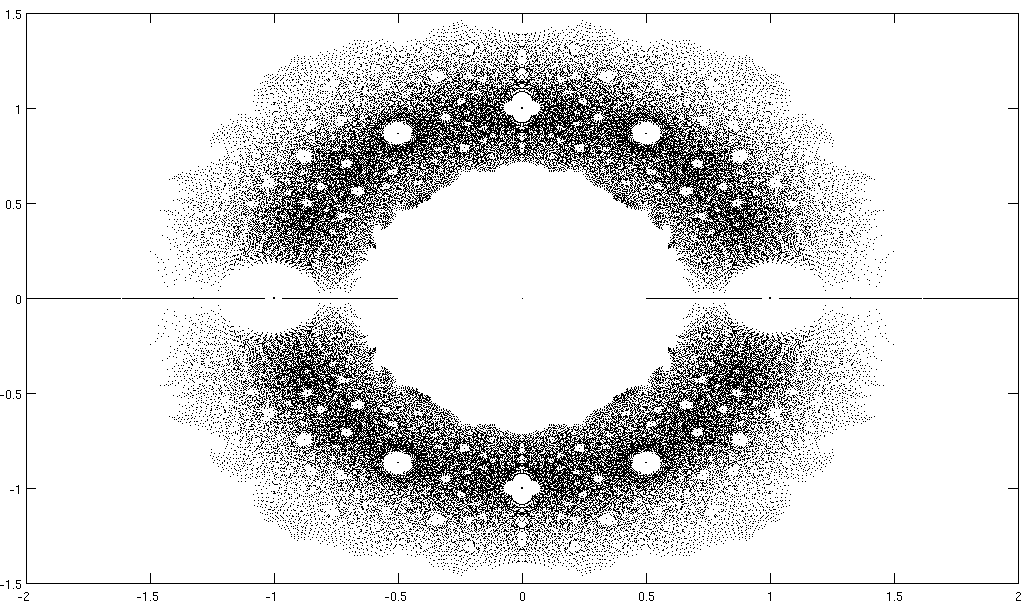
\includegraphics[width=0.8\textwidth]{zeros.png}
\label{examplefigure}
\caption{Some mathematical plot}
\end{figure}

Image courtesy of Janne Korhonen.


\end{block}
	
\end{column}

\end{columns}
\end{frame}
\end{document}